`% !TeX program = xelatex
% Editable source generated from measured project artifacts.
% Compile from this directory: tectonic 23I-2581-A2-DS-B.tex
% Or select XeLaTeX in Overleaf. Upload this file and report/images/.
\documentclass[10pt,a4paper]{article}
\usepackage[margin=12mm,top=12mm,bottom=13mm]{geometry}
\usepackage{fontspec}
\IfFontExistsTF{Arial}{\setmainfont{Arial}\setsansfont{Arial}}
  {\setmainfont{TeX Gyre Heros}\setsansfont{TeX Gyre Heros}}
\IfFontExistsTF{Consolas}{\setmonofont[Scale=.88]{Consolas}}
  {\setmonofont[Scale=.88]{Latin Modern Mono}}
\usepackage{amsmath,amssymb}
\usepackage[table]{xcolor}
\usepackage{graphicx,tabularx,booktabs,array,fancyhdr}
\usepackage{microtype}
\usepackage[hidelinks]{hyperref}
\definecolor{ink}{HTML}{18364B}
\definecolor{teal}{HTML}{008C95}
\definecolor{muted}{HTML}{5B7080}
\definecolor{pale}{HTML}{E5EFF4}
\definecolor{wash}{HTML}{F5F8FA}
\color{ink}
\setlength{\parindent}{0pt}
\setlength{\parskip}{2.5pt}
\setlength{\emergencystretch}{2em}
\setlength{\abovedisplayskip}{3pt}
\setlength{\belowdisplayskip}{3pt}
\pagestyle{fancy}\fancyhf{}
\fancyfoot[L]{\fontsize{7}{8}\selectfont\color{muted}23I-2581 · DS-B\quad / \quad THE MIDNIGHT QUEUE}
\fancyfoot[R]{\fontsize{7}{8}\selectfont\color{muted}\thepage\ / 5}
\renewcommand{\headrulewidth}{0pt}
\renewcommand{\footrulewidth}{.3pt}
\newcommand{\sectiontitle}[1]{\par\vspace{4pt}{\color{teal}\fontsize{12}{14}\selectfont\bfseries #1}\par\vspace{1pt}}
\newcommand{\subheading}[1]{\par\vspace{3pt}{\fontsize{9}{11}\selectfont\bfseries #1}\par}
\newcommand{\figcaption}[1]{\par{\fontsize{6.2}{7.1}\selectfont\color{muted}#1}\par\vspace{1pt}}
\hypersetup{pdftitle={The Midnight Queue},pdfauthor={23I-2581},
pdfsubject={Design and Analysis of Algorithms - Assignment 2}}
\begin{document}
\fontsize{8.6}{10.7}\selectfont


{\fontsize{24}{26}\selectfont\bfseries The Midnight Queue}\par
{\fontsize{11}{14}\selectfont\color{muted}Ranking suspicious transactions at scale}\par
\vspace{4pt}{\color{teal}\hrule height 1.2pt}\vspace{4pt}

{\fontsize{7.2}{9}\selectfont\color{muted}Design and Analysis of Algorithms \,\textbullet\, Assignment 2 \,\textbullet\, \textbf{Roll 23I-2581 \,\textbullet\, Section DS-B \,\textbullet\, seed 232581 \,\textbullet\, K = 52}\newline 
Intel(R) Core(TM) i7-10610U CPU @ 1.80GHz (4 physical / 8 logical cores), 31.8 GiB RAM, Windows-11-10.0.26200-SP0; Python 3.14.0, NumPy 2.4.3, pandas 3.0.1. All timed values are medians of five completed runs. The Kaggle ULB file has 284,807 rows and 492 fraud labels; it is not redistributed.}\par

\textbf{Headline.} The raw file is Time-ordered but is not triaged: only 50.6\% of adjacent pairs are in triage order, with 20.30 billion inversions. Bands 2--9 occur; 426 of 492 frauds lie in bands 6--9 and no fraud lies below band 3. The smallest queue capturing half of all frauds is \textbf{K = 2,068}. The full sort, the K=52 shift queue and the live refresh are compared on measured time, comparisons, moves and peak extra memory; DNF is reported as DNF, never as zero.\par

\sectiontitle{A. Know Your Data}

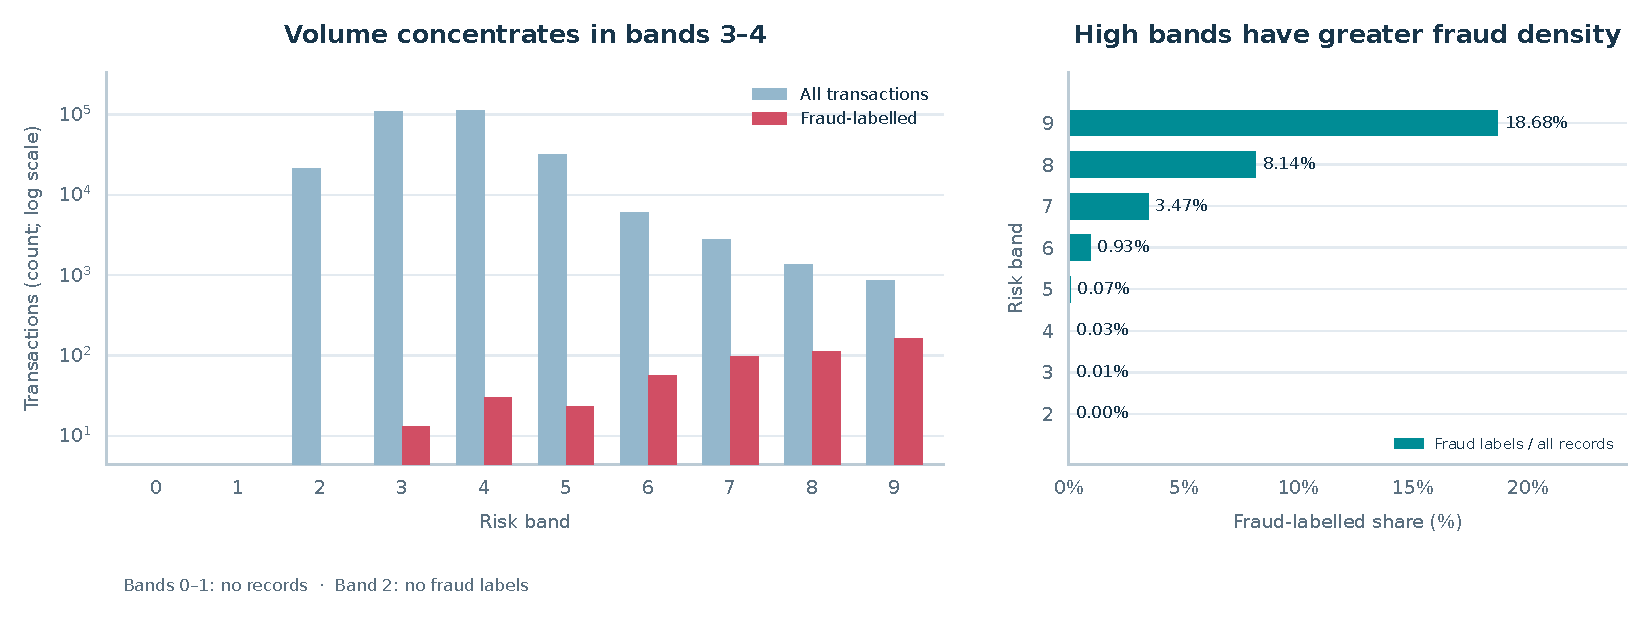
\includegraphics[width=.96\linewidth]{report/images/07_band_distribution.pdf}\par
{\fontsize{7.2}{8.496}\selectfont
\setlength{\tabcolsep}{2pt}\renewcommand{\arraystretch}{1.06}
\begin{tabularx}{\linewidth}{@{}>{\hsize=0.7500\hsize\linewidth=\hsize\raggedright\arraybackslash}X>{\hsize=1.3026\hsize\linewidth=\hsize\raggedright\arraybackslash}X>{\hsize=0.9474\hsize\linewidth=\hsize\raggedright\arraybackslash}X>{\hsize=0.7500\hsize\linewidth=\hsize\raggedright\arraybackslash}X>{\hsize=1.3026\hsize\linewidth=\hsize\raggedright\arraybackslash}X>{\hsize=0.9474\hsize\linewidth=\hsize\raggedright\arraybackslash}X@{}}
\toprule\rowcolor{pale}
\textbf{Band} & \textbf{All} & \textbf{Frauds} & \textbf{Band} & \textbf{All} & \textbf{Frauds} \\
\midrule
0 & 0 & 0 & 5 & 32,084 & 23 \\
1 & 0 & 0 & 6 & 6,006 & 56 \\
\rowcolor{wash}
2 & 21,156 & 0 & 7 & 2,797 & 97 \\
3 & 107,410 & 13 & 8 & 1,376 & 112 \\
\rowcolor{wash}
4 & 113,116 & 30 & 9 & 862 & 161 \\
\bottomrule
\end{tabularx}}\par\vspace{3pt}

\figcaption{Table A1 / Fig. A1. Band counts (all rows) and fraud labels; the histogram repeats the same data on a log count axis. Units: transactions per band. Class is read only after scoring.}

\textbf{Amount ties.} There are 32,767 distinct Amount values; the ten most frequent hold 16.29\% of rows. The mode is 1.00 (13,688 rows), so Amount alone is not a tie-breaker; the complete four-field triage key is necessary. Frauds by band are 13, 30, 23, 56, 97, 112 and 161 in bands 3--9.\par

\textbf{Which Section 3.4 properties does the raw file already have?} Its Time column is non-decreasing and its rows are in txn\_id order, so it is exactly C1 (and supplies C6's input sequence). It is not C3: only 50.6\% of adjacent pairs are in triage order versus 67.4\% for band alone, with 20.303B triage inversions. C2 and C5 require seeded construction; C4 is the exact reverse of C3; C6 changes the comparator to band alone.\par

\sectiontitle{B. Build the Contenders}

The package \texttt{src/midnight\_\allowbreak{}queue/} contains Insertion Sort (in-place shifting), top-down stable Merge Sort, Naive Quick Sort (last-pivot Lomuto, iterative stack), Hardened Quick Sort (median-of-three, three-way partition and a depth-limited in-place heap fallback), bottom-up Heap Sort, a size-K heap selector (the root is the worst retained case: a min-heap on the score with the descending comparator reversed), a bounded insertion buffer with binary search and explicit shifting, and all three live-feed strategies. No built-in or NumPy sort appears inside a contender; \texttt{sorted()} is confined to the labelled reference/verification code and to deterministic input preparation. A key comparison is one call to the central \texttt{TriageOrder.cmp}; a move is one record assignment (a swap is three). Full-sort/Top-K timers exclude CSV I/O, risk scoring, condition construction, input copying and verification. The fallback guarantees worst-case O(n log n) time without altering the required naive Lomuto contender.\par

\textbf{Correctness and the C6 clash.} The automated suite has 91 passing tests, including empty input, one record, all-equal keys, duplicate-heavy input, every condition and size, Class perturbation, Top-K boundaries and live-feed publication. C1--C5 use a total key and are checked for exact sequence equality with the reference. C6 is defined by the PDF as \textit{band alone}, so it has huge ties; a literal C6 result is checked as a permutation with non-increasing bands and no access to Amount, Time, txn\_id or Class. Band-only comparison does not define a unique row sequence; a full-key reference would impose extra criteria. This is the disclosed specification clash. The literal band-only comparator is retained and tested without secondary-field access. Conditions are C1 arrival, C2 seeded shuffle, C3 pre-ranked, C4 reverse-ranked, C5 with floor(0.01n) records deranged, C6 band-only.\par

\vspace{2pt}

\subheading{Recommendations at a glance}

{\fontsize{6.5}{7.67}\selectfont
\setlength{\tabcolsep}{2pt}\renewcommand{\arraystretch}{1.06}
\begin{tabularx}{\linewidth}{@{}>{\hsize=0.5342\hsize\linewidth=\hsize\raggedright\arraybackslash}X>{\hsize=0.5753\hsize\linewidth=\hsize\raggedright\arraybackslash}X>{\hsize=1.8904\hsize\linewidth=\hsize\raggedright\arraybackslash}X@{}}
\toprule\rowcolor{pale}
\textbf{Job} & \textbf{Ship} & \textbf{Measured evidence} \\
\midrule
Overnight batch & Merge Sort & lowest full-size worst case: 11.29 s \\
K=52 shift queue & Size-K Heap & wins 25/28 cells; max regret 1.12x \\
\rowcolor{wash}
Live refresh & Maintained heap & 0.284 s (60 min), 0.538 s (10 min) \\
\bottomrule
\end{tabularx}}\par\vspace{2pt}

\figcaption{These choices, their assumptions and the conditions that would reverse them are argued in Section H.}

\newpage
\fontsize{7.7}{9.4}\selectfont

\sectiontitle{C. The Full Ranking Tournament}

Five contenders x six conditions x four sizes: 105 valid medians and 15 DNFs cover all 120 cells. Current completed cells were remeasured with five isolated repetitions, fresh copies outside the timer, and up to four concurrent cells using exclusive requested logical-CPU slots. Algorithm-only deadlines exclude preparation and verification. Historical DNF evidence for unchanged quadratic contenders is retained and identified in the raw notes. The shared legend applies to all six panels.\par

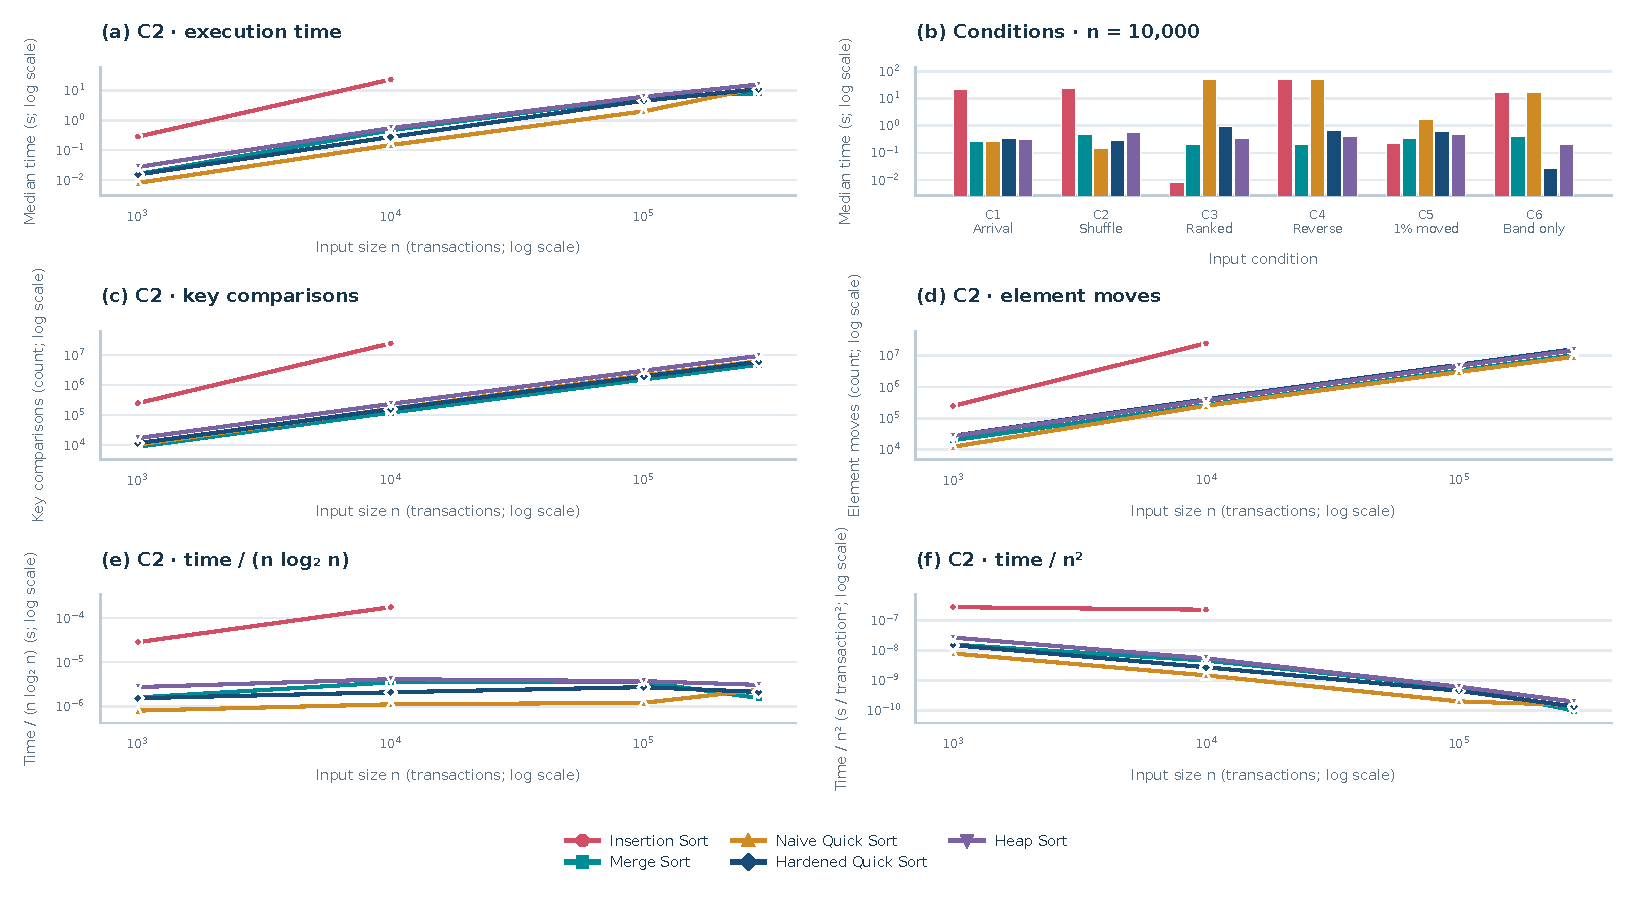
\includegraphics[width=.98\linewidth]{report/images/report_C_tournament.pdf}\par

\figcaption{Fig. C1. (a) Median time vs n on C2, log--log (s vs transactions); (b) median time at n=10,000 by condition, log scale (s); (c) comparisons and (d) moves vs n on C2, log scale (counts); (e) time/(n log2 n) and (f) time/n\(^{2}\) on C2. Missing points are DNF. The shared legend below the figure applies to all six panels.}

\textbf{What happened at n=10,000 (fastest / slowest):} C1: Merge Sort / Insertion Sort; C2: Naive Quick Sort / Insertion Sort; C3: Insertion Sort / Naive Quick Sort; C4: Merge Sort / Naive Quick Sort; C5: Insertion Sort / Naive Quick Sort; C6: Hardened Quick Sort / Insertion Sort. Insertion Sort is linear on pre-ranked C3 but quadratic on C4; the reverse and duplicate-heavy cases separate n log n from quadratic behaviour. On C5, 1\% displacement already creates 34,333,390 inversions at n=100,000.\par

\textbf{Theory versus measurement.} At 10k, insertion C1/C4 makes 24,987,904/49,995,000 comparisons, with medians 22.36 s/48.98 s; counts match the inversion model. Clash: Heap/C1 falls from 12.71 s at 100k to 9.72 s at full size while comparisons rise 3.02M to 9.44M. Power/scheduling was uncontrolled; growth conclusions use counts, and recommendations use these observed medians.\par

\begin{minipage}[t]{0.485\linewidth}\vspace{0pt}
{\fontsize{6.4}{7.552}\selectfont
\setlength{\tabcolsep}{2pt}\renewcommand{\arraystretch}{1.06}
\begin{tabularx}{\linewidth}{@{}>{\hsize=1.9600\hsize\linewidth=\hsize\raggedright\arraybackslash}X>{\hsize=0.8400\hsize\linewidth=\hsize\raggedright\arraybackslash}X>{\hsize=0.8400\hsize\linewidth=\hsize\raggedright\arraybackslash}X>{\hsize=0.8400\hsize\linewidth=\hsize\raggedright\arraybackslash}X>{\hsize=0.8400\hsize\linewidth=\hsize\raggedright\arraybackslash}X>{\hsize=0.8400\hsize\linewidth=\hsize\raggedright\arraybackslash}X>{\hsize=0.8400\hsize\linewidth=\hsize\raggedright\arraybackslash}X@{}}
\toprule\rowcolor{pale}
\textbf{Contender} & \textbf{C1} & \textbf{C2} & \textbf{C3} & \textbf{C4} & \textbf{C5} & \textbf{C6} \\
\midrule
\shortstack[l]{Insertion Sort\\ \strut} & \shortstack[l]{22.36 s\\ \strut} & \shortstack[l]{23.30 s\\ \strut} & \shortstack[l]{0.008 s\\ \strut} & \shortstack[l]{48.98 s\\ \strut} & \shortstack[l]{0.229 s\\ \strut} & \shortstack[l]{17.01 s\\ \strut} \\
\shortstack[l]{Merge Sort\\ \strut} & \shortstack[l]{0.251 s\\ \strut} & \shortstack[l]{0.465 s\\ \strut} & \shortstack[l]{0.209 s\\ \strut} & \shortstack[l]{0.206 s\\ \strut} & \shortstack[l]{0.348 s\\ \strut} & \shortstack[l]{0.403 s\\ \strut} \\
\rowcolor{wash}
\shortstack[l]{Naive Quick Sort\\ \strut} & \shortstack[l]{0.257 s\\ \strut} & \shortstack[l]{0.149 s\\ \strut} & \shortstack[l]{50.55 s\\ \strut} & \shortstack[l]{49.37 s\\ \strut} & \shortstack[l]{1.71 s\\ \strut} & \shortstack[l]{16.67 s\\ \strut} \\
\shortstack[l]{Hardened Quick Sort\\ \strut} & \shortstack[l]{0.323 s\\ \strut} & \shortstack[l]{0.277 s\\ \strut} & \shortstack[l]{0.902 s\\ \strut} & \shortstack[l]{0.677 s\\ \strut} & \shortstack[l]{0.607 s\\ \strut} & \shortstack[l]{0.027 s\\ \strut} \\
\rowcolor{wash}
\shortstack[l]{Heap Sort\\ \strut} & \shortstack[l]{0.296 s\\ \strut} & \shortstack[l]{0.550 s\\ \strut} & \shortstack[l]{0.339 s\\ \strut} & \shortstack[l]{0.386 s\\ \strut} & \shortstack[l]{0.469 s\\ \strut} & \shortstack[l]{0.195 s\\ \strut} \\
\bottomrule
\end{tabularx}}
\end{minipage}
\hfill
\begin{minipage}[t]{0.485\linewidth}\vspace{0pt}
{\fontsize{6.4}{7.552}\selectfont
\setlength{\tabcolsep}{2pt}\renewcommand{\arraystretch}{1.06}
\begin{tabularx}{\linewidth}{@{}>{\hsize=1.0000\hsize\linewidth=\hsize\raggedright\arraybackslash}X>{\hsize=1.0000\hsize\linewidth=\hsize\raggedright\arraybackslash}X>{\hsize=1.0000\hsize\linewidth=\hsize\raggedright\arraybackslash}X>{\hsize=1.0000\hsize\linewidth=\hsize\raggedright\arraybackslash}X>{\hsize=1.0000\hsize\linewidth=\hsize\raggedright\arraybackslash}X>{\hsize=1.0000\hsize\linewidth=\hsize\raggedright\arraybackslash}X@{}}
\toprule\rowcolor{pale}
\textbf{C1} & \textbf{C2} & \textbf{C3} & \textbf{C4} & \textbf{C5} & \textbf{C6} \\
\midrule
\shortstack[l]{24.99M\,/\\ 24.99M} & \shortstack[l]{24.75M\,/\\ 24.75M} & \shortstack[l]{10.0k\,/\\ 10.0k} & \shortstack[l]{49.99M\,/\\ 50.00M} & \shortstack[l]{336.0k\,/\\ 336.0k} & \shortstack[l]{17.35M\,/\\ 17.35M} \\
\shortstack[l]{120.1k\,/\\ 267.2k} & \shortstack[l]{120.5k\,/\\ 267.2k} & \shortstack[l]{64.6k\,/\\ 267.2k} & \shortstack[l]{69.0k\,/\\ 267.2k} & \shortstack[l]{91.6k\,/\\ 267.2k} & \shortstack[l]{114.2k\,/\\ 267.2k} \\
\rowcolor{wash}
\shortstack[l]{153.1k\,/\\ 201.0k} & \shortstack[l]{161.9k\,/\\ 250.8k} & \shortstack[l]{49.99M\,/\\ 0} & \shortstack[l]{49.99M\,/\\ 15.0k} & \shortstack[l]{1.30M\,/\\ 70.1k} & \shortstack[l]{16.02M\,/\\ 33.4k} \\
\shortstack[l]{152.2k\,/\\ 389.0k} & \shortstack[l]{157.4k\,/\\ 404.4k} & \shortstack[l]{323.3k\,/\\ 754.4k} & \shortstack[l]{323.3k\,/\\ 769.4k} & \shortstack[l]{233.9k\,/\\ 582.6k} & \shortstack[l]{17.5k\,/\\ 22.5k} \\
\rowcolor{wash}
\shortstack[l]{235.4k\,/\\ 371.7k} & \shortstack[l]{235.3k\,/\\ 372.7k} & \shortstack[l]{244.5k\,/\\ 395.9k} & \shortstack[l]{226.7k\,/\\ 350.1k} & \shortstack[l]{244.4k\,/\\ 394.9k} & \shortstack[l]{188.5k\,/\\ 286.5k} \\
\bottomrule
\end{tabularx}}
\end{minipage}\par\vspace{3pt}

\figcaption{Table C1 (left). Median time (s) at n=10,000; DNF is a genuine 300 s timeout. Table C2 (right). Key comparisons / element moves for the same cells, in the same row order. Counts are deterministic across repetitions.}

{\fontsize{6.5}{7.67}\selectfont
\setlength{\tabcolsep}{2pt}\renewcommand{\arraystretch}{1.06}
\begin{tabularx}{\linewidth}{@{}>{\hsize=2.1176\hsize\linewidth=\hsize\raggedright\arraybackslash}X>{\hsize=0.8517\hsize\linewidth=\hsize\raggedright\arraybackslash}X>{\hsize=0.8517\hsize\linewidth=\hsize\raggedright\arraybackslash}X>{\hsize=0.8517\hsize\linewidth=\hsize\raggedright\arraybackslash}X>{\hsize=0.8517\hsize\linewidth=\hsize\raggedright\arraybackslash}X>{\hsize=0.8517\hsize\linewidth=\hsize\raggedright\arraybackslash}X>{\hsize=0.8517\hsize\linewidth=\hsize\raggedright\arraybackslash}X>{\hsize=0.8977\hsize\linewidth=\hsize\raggedright\arraybackslash}X>{\hsize=0.8747\hsize\linewidth=\hsize\raggedright\arraybackslash}X@{}}
\toprule\rowcolor{pale}
\textbf{Contender} & \textbf{C1} & \textbf{C2} & \textbf{C3} & \textbf{C4} & \textbf{C5} & \textbf{C6} & \textbf{Stable} & \textbf{Space} \\
\midrule
Insertion Sort & 0 B & 0 B & 0 B & 0 B & 0 B & 0 B & yes & O(1) \\
Merge Sort & 79.0 KiB & 79.0 KiB & 79.0 KiB & 79.0 KiB & 79.0 KiB & 79.0 KiB & yes & O(n) \\
\rowcolor{wash}
Naive Quick Sort & 64 B & 64 B & 32 B & 32 B & 64 B & 32 B & no & O(log n)* \\
Hardened Quick Sort & 64 B & 64 B & 392 B & 392 B & 392 B & 32 B & no & O(log n) \\
\rowcolor{wash}
Heap Sort & 0 B & 0 B & 0 B & 0 B & 0 B & 0 B & no & O(1) \\
\bottomrule
\end{tabularx}}\par\vspace{2pt}

\figcaption{Table C3. tracemalloc peak extra memory at n=10,000 (KiB or B), peak values are per cell; stability and asymptotic space. *The iterative naive quick sort processes the smaller side first, so its explicit stack is O(log n) in practice even on bad splits.}

{\fontsize{6.5}{7.67}\selectfont
\setlength{\tabcolsep}{2pt}\renewcommand{\arraystretch}{1.06}
\begin{tabularx}{\linewidth}{@{}>{\hsize=1.0000\hsize\linewidth=\hsize\raggedright\arraybackslash}X>{\hsize=0.8000\hsize\linewidth=\hsize\raggedright\arraybackslash}X>{\hsize=0.8000\hsize\linewidth=\hsize\raggedright\arraybackslash}X>{\hsize=1.1500\hsize\linewidth=\hsize\raggedright\arraybackslash}X>{\hsize=1.2500\hsize\linewidth=\hsize\raggedright\arraybackslash}X@{}}
\toprule\rowcolor{pale}
\textbf{Cell} & \textbf{Largest completed} & \textbf{t at completed} & \textbf{Projection 100k} & \textbf{Projection full} \\
\midrule
Insertion / C1 & 10,000 & 22.36 s & 37.27 min & 302.30 min \\
Insertion / C2 & 10,000 & 23.30 s & 38.83 min & 315.01 min \\
\rowcolor{wash}
Insertion / C4 & 10,000 & 48.98 s & 81.63 min & 662.11 min \\
Insertion / C5 & 100,000 & 29.31 s & 29.31 s & 3.96 min \\
\rowcolor{wash}
Insertion / C6 & 10,000 & 17.01 s & 28.35 min & 229.98 min \\
Naive Quick / C3 & 10,000 & 50.55 s & 84.25 min & 683.42 min \\
\rowcolor{wash}
Naive Quick / C4 & 10,000 & 49.37 s & 82.29 min & 667.51 min \\
Naive Quick / C6 & 10,000 & 16.67 s & 27.78 min & 225.32 min \\
\bottomrule
\end{tabularx}}\par\vspace{2pt}

\figcaption{Table C4. Largest completed sizes and explicit quadratic projections from their measured medians. Projections are not observations; DNFs have no median. All raw repetitions are in results.csv.}

\newpage
\fontsize{7.5}{9.1}\selectfont

\sectiontitle{D. The Shift Queue (Top-K)}

Three custom ways produce the same ordered queue: hardened full sort plus the K-prefix, a size-K heap with its worst retained case at the root, and a bounded binary-search insertion buffer. The heap is a min-heap of priority (band, Amount, -Time, -txn\_id), equivalently a max-heap under the best-first comparator. The full sort is now measured at every K, including its actual prefix copy. Heap/buffer comparison loops are unchanged; their earlier five-run measurements remain identified by provenance. The grid is K=\{10,50,52,500,2068,5000,n/10\}, both required sizes and C1/C2. Class is evaluated only after ranking.\par

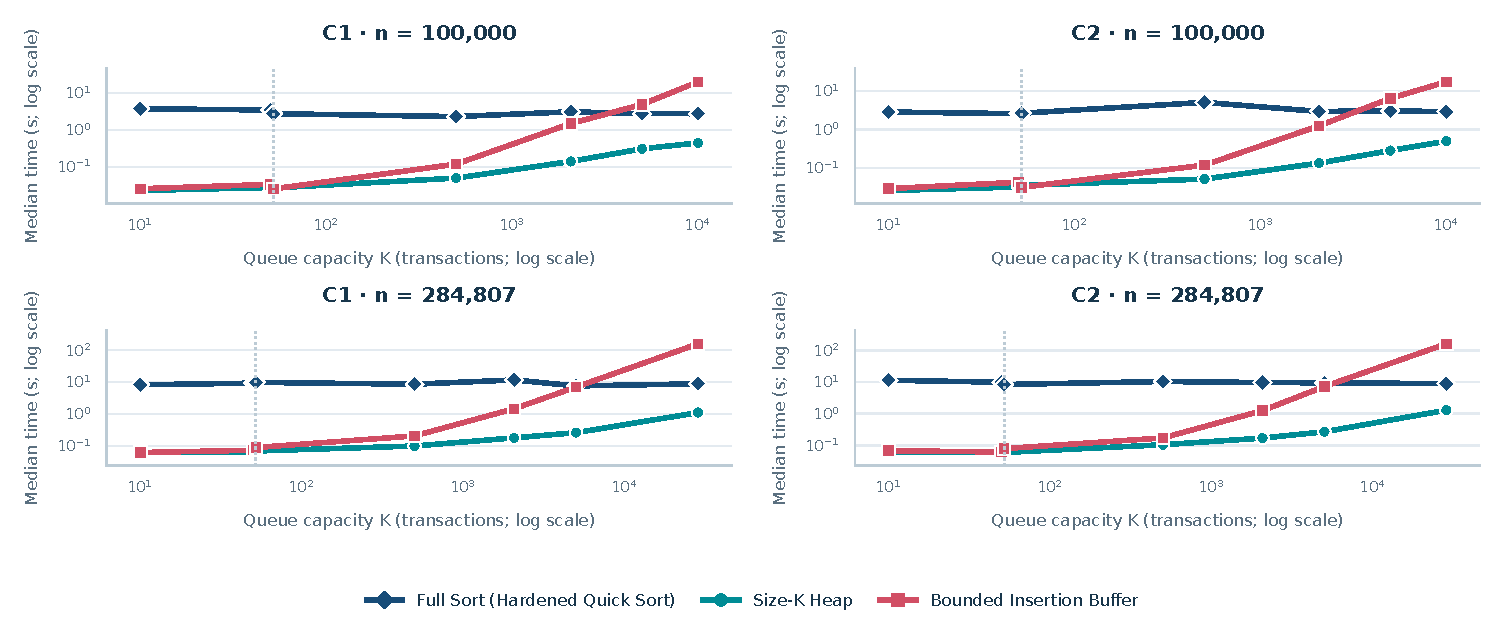
\includegraphics[width=.98\linewidth]{report/images/report_D_topk.pdf}\par

\figcaption{Fig. D1. Median cost of a complete ordered K-queue, log--log (s vs K); C1 and C2 at n=100,000 and 284,807. DNF is omitted, not interpolated.}

\begin{minipage}[t]{0.485\linewidth}\vspace{0pt}
{\fontsize{6.4}{7.552}\selectfont
\setlength{\tabcolsep}{2pt}\renewcommand{\arraystretch}{1.06}
\begin{tabularx}{\linewidth}{@{}>{\hsize=0.8258\hsize\linewidth=\hsize\raggedright\arraybackslash}X>{\hsize=0.6607\hsize\linewidth=\hsize\raggedright\arraybackslash}X>{\hsize=1.1712\hsize\linewidth=\hsize\raggedright\arraybackslash}X>{\hsize=1.1712\hsize\linewidth=\hsize\raggedright\arraybackslash}X>{\hsize=1.1712\hsize\linewidth=\hsize\raggedright\arraybackslash}X@{}}
\toprule\rowcolor{pale}
\textbf{n} & \textbf{K} & \textbf{Full sort} & \textbf{Size-K heap} & \textbf{Buffer} \\
\midrule
100,000 & 52 & 2.64 s & 0.035 s & 0.032 s \\
100,000 & 2,068 & 2.92 s & 0.134 s & 1.24 s \\
\rowcolor{wash}
100,000 & 10,000 & 2.89 s & 0.498 s & 17.16 s \\
284,807 & 52 & 8.35 s & 0.059 s & 0.079 s \\
\rowcolor{wash}
284,807 & 2,068 & 9.65 s & 0.170 s & 1.25 s \\
284,807 & 28,480 & 8.94 s & 1.29 s & 2.69 min \\
\bottomrule
\end{tabularx}}
\end{minipage}
\hfill
\begin{minipage}[t]{0.485\linewidth}\vspace{0pt}
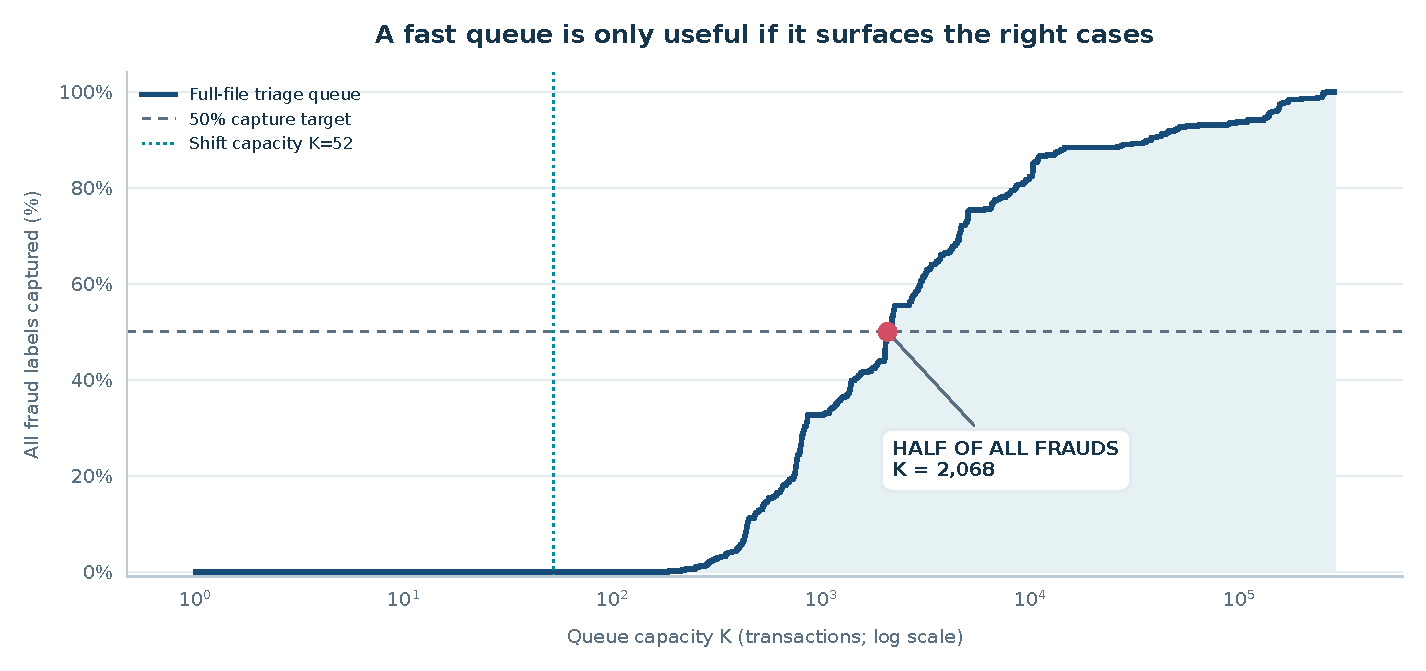
\includegraphics[width=\linewidth]{report/images/08_fraud_capture.pdf}
\end{minipage}\par\vspace{3pt}

\figcaption{Table D1 / Fig. D2. C2 queue cost at K=52, K=2,068 and K=n/10; fraud capture vs K over all 492 frauds. Class is never a sort key.}

\textbf{Fraud capture.} K=52 captures 0 of 492 frauds; the minimum half-capture queue is K=2,068. K=500 captures 63, K=5,000 captures 361, and K=10,000 captures 405. Over 28 measured grid cells, the size-K heap wins 25; its worst regret is 1.12x. The buffer wins only C1/100k/K=52, C2/100k/K=52, C1/full/K=10; full sort wins no measured cell. A small computationally cheap queue can still miss every fraud: capacity and ranking quality must be justified separately.\par

\sectiontitle{E. The Live Feed}

Consecutive Time windows start at the first transaction. After each window, each strategy publishes the top K of all records seen: A re-ranks the prefix, B updates its maintained heap, C sorts the new window and merges its ranked candidates. Every publication is verified after its timer stops. All strategies were remeasured in this revision. Simulation totals and curves now use the same sum of algorithm-only window times; five individual totals are retained. Memory is measured separately.\par

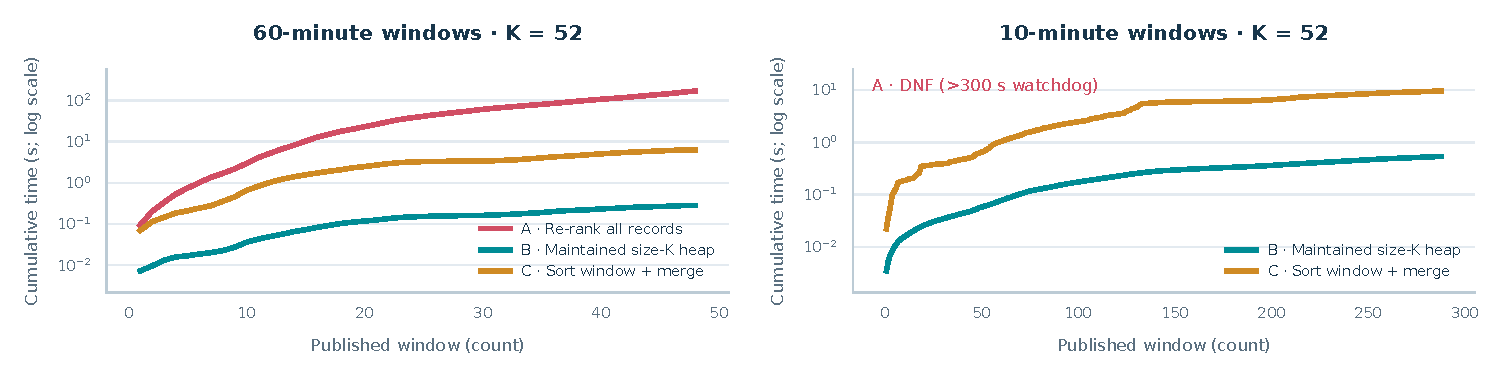
\includegraphics[width=.98\linewidth]{report/images/report_E_livefeed.pdf}\par

\figcaption{Fig. E1. Median cumulative algorithm time at each publication across five completed simulations; left: 60-minute windows, right: 10-minute windows, K=52. Only completed five-run strategies have curves. The vertical axes use logarithmic seconds so all completed strategies remain visible.}

\begin{minipage}[t]{0.485\linewidth}\vspace{0pt}
{\fontsize{6.4}{7.552}\selectfont
\setlength{\tabcolsep}{2pt}\renewcommand{\arraystretch}{1.06}
\begin{tabularx}{\linewidth}{@{}>{\hsize=0.7903\hsize\linewidth=\hsize\raggedright\arraybackslash}X>{\hsize=1.1185\hsize\linewidth=\hsize\raggedright\arraybackslash}X>{\hsize=1.0456\hsize\linewidth=\hsize\raggedright\arraybackslash}X>{\hsize=1.0456\hsize\linewidth=\hsize\raggedright\arraybackslash}X@{}}
\toprule\rowcolor{pale}
\textbf{Window} & \textbf{A: re-rank} & \textbf{B: heap} & \textbf{C: merge} \\
\midrule
60 min & 2.84 min & 0.284 s & 6.36 s \\
10 min & DNF & 0.538 s & 9.61 s \\
\bottomrule
\end{tabularx}}
\end{minipage}
\hfill
\begin{minipage}[t]{0.485\linewidth}\vspace{0pt}
{\fontsize{6.4}{7.552}\selectfont
\setlength{\tabcolsep}{2pt}\renewcommand{\arraystretch}{1.06}
\begin{tabularx}{\linewidth}{@{}>{\hsize=0.7903\hsize\linewidth=\hsize\raggedright\arraybackslash}X>{\hsize=1.1185\hsize\linewidth=\hsize\raggedright\arraybackslash}X>{\hsize=1.0456\hsize\linewidth=\hsize\raggedright\arraybackslash}X>{\hsize=1.0456\hsize\linewidth=\hsize\raggedright\arraybackslash}X@{}}
\toprule\rowcolor{pale}
\textbf{Window} & \textbf{A peak} & \textbf{B peak} & \textbf{C peak} \\
\midrule
60 min & 6.69 MiB & 31.6 KiB & 4.43 MiB \\
10 min & - & 210.6 KiB & 2.57 MiB \\
\bottomrule
\end{tabularx}}
\end{minipage}\par\vspace{3pt}

\figcaption{Table E1: median of five algorithm-only simulation totals. Table E2: peak extra memory in a separate trace. Shared windows are prepared before tracing. Retained measurement rows add O(w) bookkeeping to the streaming heap's O(K) algorithmic state. A timed-out strategy has no median.}

\newpage
\fontsize{8.1}{9.8}\selectfont

\sectiontitle{F. The Mathematical Case}

\textbf{M1 --- Insertion Sort.} If \(I\) is the inversion count, every
    shift removes one inversion: moves \(=I+n-1\), comparisons
    \(=I+n-1-z\), with \(0\leq z\leq n-1\). Thus \(T(n,I)=\Theta(n+I)\).
    Best: \(I=0\), \(\Theta(n)\); random distinct keys:
    \(\mathbb E[I]=n(n-1)/4\), \(\Theta(n^2)\); reverse:
    \(I=n(n-1)/2\), \(\Theta(n^2)\). C5 inversion counts at the four sizes:
    \(3{,}007;\ 325{,}988;\ 34{,}333{,}390;\ 272{,}954{,}546\).
    Moving only 1\% of records does not guarantee linear work.\par

\textbf{M2 --- Merge Sort.} Iterating
    \(T(n)=2T(n/2)+cn\) gives
    \(T(n)=2^jT(n/2^j)+jcn\).
    At \(j=\log_2n\), this is \(nT(1)+cn\log_2n=\Theta(n\log n)\).
    Master's theorem: \(a=b=2\), \(f(n)=\Theta(n^{\log_ba})=\Theta(n)\);
    case 2 confirms \(\Theta(n\log n)\).\par

\textbf{M3 --- Quick Sort.} (a) Iteration of
    \(T(n)=T(n-1)+cn\) yields
    \(T(1)+c\sum_{j=2}^{n}j=\Theta(n^2)\).
    (b) The balanced recursion tree has \(\log_2n\) levels of
    \(\Theta(n)\) work, hence \(\Theta(n\log n)\).
    (c) For \(T(n)=T(n/10)+T(9n/10)+n\), each complete level conserves
    total size \(n\). The first \(\lfloor\log_{10}n\rfloor\) levels give
    \(\Omega(n\log n)\); depth is at most
    \(\lceil\log_{10/9}n\rceil\), giving \(O(n\log n)\).
    Together these prove the tight bound \(\Theta(n\log n)\).\par

\textbf{M4 --- Heap Sort.} A height-\(h\) node costs \(O(h)\)
    to sift, and there are at most \(\lceil n/2^{h+1}\rceil\) such nodes.
    Bottom-up build costs
    \(O(n\sum_{h\geq0}h/2^{h+1})=O(n)\); visiting the internal nodes gives
    \(\Omega(n)\), so build is \(\Theta(n)\).
    Each of \(n-1\) extractions costs \(O(\log n)\);
    total worst-case time is \(\Theta(n\log n)\), with \(O(1)\) auxiliary space.\par

\textbf{M5 --- Top-K.}
                    For \(2\leq K\leq n\), full sort and prefix costs \(\Theta(n\log n)\).
                    For the heap, bottom-up build is \(O(K)\), scanning is
                    \(O(n+A\log K)\) for \(A\) accepted replacements, and
                    ordered publication is \(O(K\log K)\); worst case
                    \(O(n\log K+K\log K)\).
                    The buffer costs \(O(K\log K+n+A(K+\log K))\):
                    rejected records need one comparison, accepted records need
                    binary search and explicit shifting. Worst case \(O(nK)\);
                    for a random permutation of distinct keys, record \(i>K\)
                    enters with probability \(K/i\), so \(\mathbb E[A]=K(H_n-H_K)\),
                    where \(H_j\) is the \(j\)-th harmonic number.
                    An idealised comparison equates
                    \((n+K)\log_2K=n\log_2n\); actual crossover depends on
                    constants, arrival order and acceptance rate, and is not
                    established beyond the measured grid. The prediction that full sort overtakes near K=10,000 at n=100,000 was wrong on C2: heap 0.498 s, full sort 2.89 s. At full size and K=n/10=28,480: heap 1.29 s, full sort 8.94 s. These are measured points, not a universal crossover.\par

{\fontsize{6.2}{7.316}\selectfont
\setlength{\tabcolsep}{2pt}\renewcommand{\arraystretch}{1.06}
\begin{tabularx}{\linewidth}{@{}>{\hsize=0.4825\hsize\linewidth=\hsize\raggedright\arraybackslash}X>{\hsize=2.1930\hsize\linewidth=\hsize\raggedright\arraybackslash}X>{\hsize=0.7895\hsize\linewidth=\hsize\raggedright\arraybackslash}X>{\hsize=0.8333\hsize\linewidth=\hsize\raggedright\arraybackslash}X>{\hsize=0.7018\hsize\linewidth=\hsize\raggedright\arraybackslash}X@{}}
\toprule\rowcolor{pale}
\textbf{n} & \textbf{Band groups m\_i} & \textbf{Group formula} & \textbf{Exact model} & \textbf{Measured} \\
\midrule
1,000 & 84, 371, 397, 107, 24, 8, 5, 4 & 156.7k & 158.6k & 158.6k \\
10,000 & 719, 3809, 3964, 1094, 225, 98, 59, 32 & 16.00M & 16.02M & 16.02M \\
\rowcolor{wash}
100,000 & 7399,\allowbreak 37639,\allowbreak 39769,\allowbreak 11246,\allowbreak 2152,\allowbreak 995,\allowbreak 488,\allowbreak 312 & 1.59B & not simulated & DNF \\
284,807 & 21156,\allowbreak 107410,\allowbreak 113116,\allowbreak 32084,\allowbreak 6006,\allowbreak 2797,\allowbreak 1376,\allowbreak 862 & 12.93B & not simulated & DNF \\
\bottomrule
\end{tabularx}}\par\vspace{2pt}

\figcaption{Table F1 (M6). The groups are shown in band order. Group formula \(\Sigma\) m\_i(m\_i-1)/2; the exact element model is cheap only to 10k.}

\textbf{M6 --- Naive Quick Sort on C6.}
                    A one-band subarray of size \(m\) loses one pivot each time,
                    so it costs \(\sum_{j=1}^{m-1}j=\binom m2\) comparisons.
                    Hence \(C(S)=\sum_i\binom{m_i}{2}+X(S)\), where \(X\)
                    counts cross-band comparisons and depends on the actual band sequence.
                    The exact model applies the descending-band Lomuto swaps and recurrence
                    \(C(S)=|S|-1+C(L_p(S))+C(R_p(S))\), with \(C(S)=0\) for \(|S|<2\).
                    Counts alone do not determine \(X\). At n=1,000 and 10,000, exact model = measured = 158,620 and 16,023,019. The former ascending-partition model was incorrect. The within-band terms at 100k and full size are 1.59B and 12.93B; both measured cells are DNFs. Three-way partitioning processes equal bands together.\par

\textbf{M7 --- Live feed.} For \(w\) equal-size windows and \(K\geq2\),
    the worst-case costs are
    \(T_A=\sum_{j=1}^{w}\Theta((jn/w)\log(jn/w))=\Theta(nw\log n)\);
    \(T_B=O(n\log K+wK\log K)\), including every ordered heap publication;
    and \(T_C=O(n\log(n/w)+wK)\). Comparing the selection/sorting terms gives
    the rough threshold \(w\approx n/K\): many small windows favour merge,
    fewer large windows favour the heap. This threshold ignores constants and
    publication terms, so it is a guide rather than a measured crossover.
    At \(n=284{,}807\), \(K=52\), it suggests about \(5{,}477\) windows;
    the tested 48 and 288 windows both favour the heap in the recorded data.\par

\textbf{M8 --- Space.} Insertion and Heap Sort: \(O(1)\);
    Merge Sort: \(O(n)\); both Quick Sort variants: \(O(\log n)\) explicit
    stack because the smaller side is processed first; size-\(K\) heap and
    bounded buffer: \(O(K)\). Live re-rank: \(O(n)\);
    live heap: \(O(K)\); live window merge: \(O(n/w+K)\), for equal-size windows.
    These are algorithmic auxiliary-space bounds; retained measurement logs are separate.\par

\sectiontitle{H. Recommendation to the Platform Lead}

\textbf{1. Overnight batch: ship Merge Sort.} Lowest worst completed time across C1--C5 at full size wins. Worst medians: Hardened Quick Sort: 31.13 s; Heap Sort: 15.84 s; Merge Sort: 11.29 s. Hardened Quick Sort now has an in-place heap fallback after twice the binary-log depth, guaranteeing O(n log n) worst-case time and O(log n) stack. The choice assumes the unknown next batch resembles the tested conditions; it is wrong for an already ranked batch, where insertion sort takes 0.382 s.\par

\textbf{2. Shift queue: ship Size-K Heap.} Across the 28 measured cells it minimises worst slowdown relative to the winner: Bounded Insertion Buffer: max regret 140.88x; Full Sort (Hardened Quick Sort): max regret 186.16x; Size-K Heap: max regret 1.12x. The recommendation assumes K is small relative to n and scores do not change after arrival. It can be wrong near full capacity, or for a fixed small corner where another method is a few milliseconds faster. Changing scores require an update/rebuild mechanism. The operational K=52 queue still contains no frauds; the half-capture capacity must be considered separately.\par

\textbf{3. Live refresh: ship maintained size-K heap.} Algorithm-only totals: 60 min: rerank 2.84 min, heap 0.284 s, merge 6.36 s; 10 min: rerank DNF, heap 0.538 s, merge 9.61 s. A maintained heap touches new records once and avoids re-ranking history. This assumes immutable scores and windows large enough to amortise publication. Very small windows or K near n can favour window merge. The w\(\approx\)n/K comparison is a rough guide, not a measured universal crossover.\par

\subheading{Bonus: Analyst console}

The local analyst console launches with \texttt{python scripts/run\_\allowbreak{}console.py}. Choose any of the five full sorts or either Top-K selector, set K, input size and condition, then inspect every queued transaction by paginated risk band, Amount and Time. Each run displays algorithm-only time, comparisons and moves, verifies the ordered queue, and supports cancelling its isolated worker. Single demonstration measurements are logged separately from five-run medians. It uses the same algorithms and scoring as the report.\par

\subheading{AI-use disclosure}

The original project records OpenCode with DeepSeek V4.1 Flash assistance for implementation, tests, experiment orchestration, analysis and drafting. OpenAI Codex revised visualisations, notebook presentation, compliance checks and the editable LaTeX report; then hardened quicksort, corrected the C6 model and timing scopes, expanded tests, reran affected experiments, and added the analyst console and viva practice materials. Historical measurements remain archived, including excluded over-limit C5 insertion runs. The student must verify the submission and be able to explain and modify it in the viva.\par

\newpage
\fontsize{8.8}{10.6}\selectfont

\subheading{Appendix: prediction log}

Each prediction was written before its round; outcomes were updated from the measured medians. Full rationales are in \texttt{prediction\_\allowbreak{}log.csv}. W/L = predicted or actual fastest / slowest. Abbreviations: IS insertion, MS merge, NQ naive quick, HQ hardened quick, HS heap, SH size-K heap, BB bounded buffer, FS full sort, RR re-rank, MG merge, HB maintained heap. Original forecasts and their timestamps are preserved; outcomes now use revised measurements. A vertical bar joins censored DNFs: their relative speeds are unknown. The revised campaign's prospective C forecasts are stored separately in outputs/revision/predictions.csv.\par

\begin{minipage}[t]{0.485\linewidth}\vspace{0pt}
{\fontsize{8.0}{9.44}\selectfont
\setlength{\tabcolsep}{2pt}\renewcommand{\arraystretch}{1.06}
\begin{tabularx}{\linewidth}{@{}>{\hsize=0.9070\hsize\linewidth=\hsize\raggedright\arraybackslash}X>{\hsize=0.9535\hsize\linewidth=\hsize\raggedright\arraybackslash}X>{\hsize=0.9535\hsize\linewidth=\hsize\raggedright\arraybackslash}X>{\hsize=1.1860\hsize\linewidth=\hsize\raggedright\arraybackslash}X@{}}
\toprule\rowcolor{pale}
\textbf{Tournament} & \textbf{Pred W/L} & \textbf{Actual W/L} & \textbf{Outcome} \\
\midrule
C1-1k & HQ / IS & NQ / IS & slowest correct \\
C2-1k & HQ / IS & NQ / IS & slowest correct \\
\rowcolor{wash}
C3-1k & IS / NQ & IS / NQ & both correct \\
C4-1k & HQ / IS & MS / IS & slowest correct \\
\rowcolor{wash}
C5-1k & IS / NQ & IS / NQ & both correct \\
C6-1k & HQ / NQ & HQ / NQ & both correct \\
\rowcolor{wash}
C1-10k & HQ / IS & MS / IS & slowest correct \\
C2-10k & HQ / IS & NQ / IS & slowest correct \\
\rowcolor{wash}
C3-10k & IS / NQ & IS / NQ & both correct \\
C4-10k & HQ / IS & MS / NQ & both wrong \\
\rowcolor{wash}
C5-10k & HQ / NQ & IS / NQ & slowest correct \\
C6-10k & HQ / NQ & HQ / IS & fastest correct \\
\rowcolor{wash}
C1-100k & HQ / IS & NQ / IS & slowest correct \\
C2-100k & HQ / IS & NQ / IS & slowest correct \\
\rowcolor{wash}
C3-100k & IS / NQ & IS / NQ & both correct \\
C4-100k & HQ / IS & HS / IS|NQ & loss censored \\
\rowcolor{wash}
C5-100k & HQ / NQ & MS / IS & both wrong \\
C6-100k & HQ / NQ & HQ / IS|NQ & win OK; censored \\
\rowcolor{wash}
C1-full & HQ / IS & HQ / IS & both correct \\
C2-full & HQ / IS & MS / IS & slowest correct \\
\rowcolor{wash}
C3-full & IS / NQ & IS / NQ & both correct \\
C4-full & HQ / IS & MS / IS|NQ & loss censored \\
\rowcolor{wash}
C5-full & HQ / NQ & MS / IS & both wrong \\
C6-full & HQ / NQ & HQ / IS|NQ & win OK; censored \\
\bottomrule
\end{tabularx}}
\end{minipage}
\hfill
\begin{minipage}[t]{0.485\linewidth}\vspace{0pt}
{\fontsize{8.0}{9.44}\selectfont
\setlength{\tabcolsep}{2pt}\renewcommand{\arraystretch}{1.06}
\begin{tabularx}{\linewidth}{@{}>{\hsize=1.2514\hsize\linewidth=\hsize\raggedright\arraybackslash}X>{\hsize=0.8045\hsize\linewidth=\hsize\raggedright\arraybackslash}X>{\hsize=0.8045\hsize\linewidth=\hsize\raggedright\arraybackslash}X>{\hsize=1.1397\hsize\linewidth=\hsize\raggedright\arraybackslash}X@{}}
\toprule\rowcolor{pale}
\textbf{D/E/F row} & \textbf{Pred} & \textbf{Actual} & \textbf{Outcome} \\
\midrule
M5 crossover & SH / BB & --- & see M5 \\
C1-100k/K10 & SH / BB & SH / FS & fastest correct \\
\rowcolor{wash}
C1-100k/K50 & SH / BB & SH / FS & fastest correct \\
C1-100k/K52 & SH / BB & BB / FS & both wrong \\
\rowcolor{wash}
C1-100k/K500 & SH / BB & SH / FS & fastest correct \\
C1-100k/K5000 & SH / BB & SH / BB & both correct \\
\rowcolor{wash}
C1-100k/K10000 & FS / BB & SH / BB & slowest correct \\
C1-100k/K2068 & SH / BB & SH / FS & fastest correct \\
\rowcolor{wash}
C2-100k/K10 & SH / BB & SH / FS & fastest correct \\
C2-100k/K50 & SH / BB & SH / FS & fastest correct \\
\rowcolor{wash}
C2-100k/K52 & SH / BB & BB / FS & both wrong \\
C2-100k/K500 & SH / BB & SH / FS & fastest correct \\
\rowcolor{wash}
C2-100k/K5000 & SH / BB & SH / BB & both correct \\
C2-100k/K10000 & FS / BB & SH / BB & slowest correct \\
\rowcolor{wash}
C2-100k/K2068 & SH / BB & SH / FS & fastest correct \\
C1-full/K10 & SH / BB & BB / FS & both wrong \\
\rowcolor{wash}
C1-full/K50 & SH / BB & SH / FS & fastest correct \\
C1-full/K52 & SH / BB & SH / FS & fastest correct \\
\rowcolor{wash}
C1-full/K500 & SH / BB & SH / FS & fastest correct \\
C1-full/K5000 & SH / BB & SH / FS & fastest correct \\
\rowcolor{wash}
C1-full/K28480 & FS / BB & SH / BB & slowest correct \\
C1-full/K2068 & SH / BB & SH / FS & fastest correct \\
\rowcolor{wash}
C2-full/K10 & SH / BB & SH / FS & fastest correct \\
C2-full/K50 & SH / BB & SH / FS & fastest correct \\
\rowcolor{wash}
C2-full/K52 & SH / BB & SH / FS & fastest correct \\
C2-full/K500 & SH / BB & SH / FS & fastest correct \\
\rowcolor{wash}
C2-full/K5000 & SH / BB & SH / FS & fastest correct \\
C2-full/K28480 & FS / BB & SH / BB & slowest correct \\
\rowcolor{wash}
C2-full/K2068 & SH / BB & SH / FS & fastest correct \\
live/3600 & HB / RR & HB / RR & both correct \\
\rowcolor{wash}
live/600 & HB / RR & HB / RR & both correct \\
\bottomrule
\end{tabularx}}
\end{minipage}\par\vspace{3pt}

\figcaption{Table P1. Original forecasts with revised outcomes: 24 C rounds and 31 D/E/F rows. M5 is the crossover forecast discussed in M5. DNFs have no measured times and are not ordered among themselves.}

\textbf{Artifacts.} results.csv contains 4,876 rows: 4,545 run/window rows, 25 simulation totals, 189 medians, 5 live summaries, 51 memory observations, 16 DNFs, 15 labelled quadratic projections, 7 interrupted attempts, 17 single console demonstrations and 6 excluded historical observations. The 55 original forecasts remain in prediction\_log.csv. The executed notebook demonstrates scoring, ranking correctness and fraud capture; README.md supplies reproduction commands.\par

\end{document}'